\documentclass[conference]{IEEEtran}
\IEEEoverridecommandlockouts
% The preceding line is only needed to identify funding in the first footnote. If that is unneeded, please comment it out.
\usepackage{cite}
\usepackage{amsmath,amssymb,amsfonts}
\usepackage{algorithmic}
\usepackage{graphicx}
\usepackage{textcomp}
\usepackage{hyperref}
\usepackage{xcolor}
\def\BibTeX{{\rm B\kern-.05em{\sc i\kern-.025em b}\kern-.08em
    T\kern-.1667em\lower.7ex\hbox{E}\kern-.125emX}}
\begin{document}

\title{Humanoid Sprinting and Stopping DRL}

\author{

    \IEEEauthorblockN{Carlos Veríssimo}
    \IEEEauthorblockA{\textit{Department of Informatics Engineering} \\
        \textit{FEUP}\\
        Porto, Portugal \\
        up201907716@up.pt }
    \and

    \IEEEauthorblockN{Miguel Amorim}
    \IEEEauthorblockA{\textit{Department of Informatics Engineering } \\
        \textit{FEUP}\\
        Porto, Portugal \\
        up201907756@up.pt }
    \and

    \IEEEauthorblockN{Rafael Camelo}
    \IEEEauthorblockA{\textit{Department of Informatics Engineering } \\
        \textit{FEUP}\\
        Porto, Portugal \\
        up201907729@up.pt }
}


\maketitle

\begin{abstract}

\end{abstract}

\begin{IEEEkeywords}
RoboCup, RoboCup 3D Simulation League, Reinforcement Learning, Humanoid Sprinting, Humanoid Stopping, Soccer
\end{IEEEkeywords}

\section{Introduction}

Reinforcement learning (RL) is a machine learning field in which agents learn optimal behaviours through trial-and-error interactions with their environment to maximize rewards and minimize punishments.

The RoboCup, which began in 1997, is a well-known platform for promoting robots and AI by pushing participants with tasks such as soccer, rescue, and home care. \cite{robocup97}.

This article digs into RoboCup's 3D Simulation League, introduced in 2004. The league evolved from using simple spheres to humanoid robots and now uses a simulated version of the NAO robot, a 58-cm-tall robot with 25 degrees of freedom (DOF) \cite{naorobot}, as the robot model.

\begin{figure}[htbp]
    \centerline{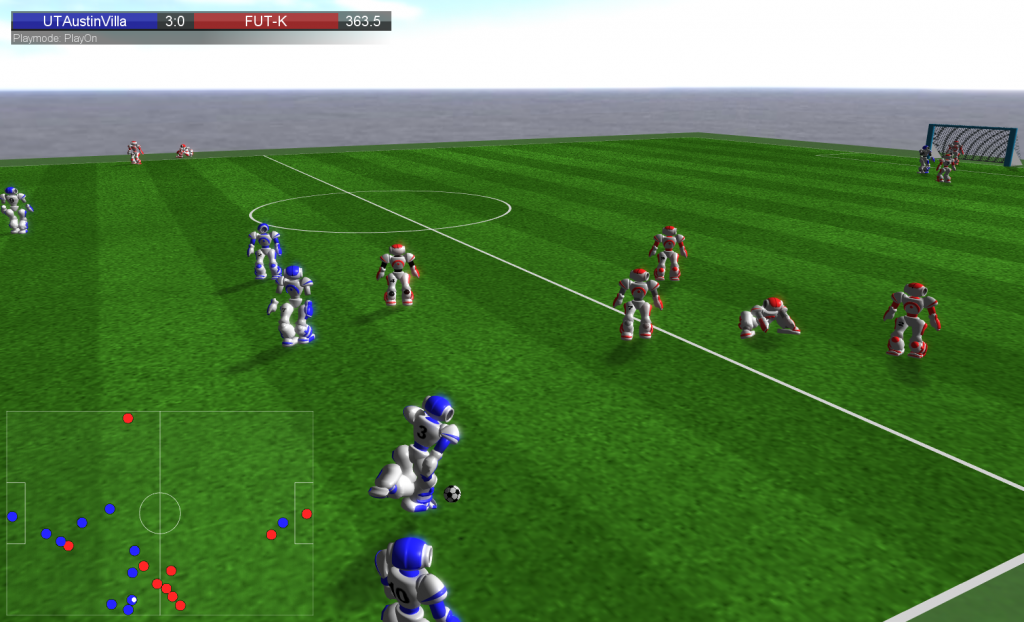
\includegraphics[width=0.35\textwidth]{images/robocup3d.png}}
    \caption{RoboCup 3D Simulation League.}
    \label{fig:robocup3d}
\end{figure}

To enforce physics laws, coordinate communications between the server and clients, and officiate the game, the league uses the SimSpark simulator.

Sprinting is an important feature of robotic soccer and plays a key role in team success. This paper also focuses on the difficult problem of stopping a run without falling, a feat that necessitates detailed control over the robot's numerous joints and sensors.

This study focuses on improving humanoid robot running and halting in the RoboCup 3D Simulation League.
Recognizing the intricacy and significance of these talents in robotic soccer, we intend to expand on previous advances in the field.
Our primary goal is to create solid, reliable techniques for accelerating and decelerating without falling by making use of comprehensive control
of the robot's joints and sensors.

Subsequent sections detail related works (Section \ref{Related Work}), our methodology (Section \ref{Methodology}),
the significant results and their implications (Section \ref{Results and Discussion}),
concluding with future directions for this field (Section \ref{Conclusions and Future Work})

\section{Related Work}\label{Related Work}

Yearly held in different countries, the RoboCup, and, in particular, its 3D Simulated Soccer League, has been a platform for the development of new techniques and algorithms in the field of robotics and artificial intelligence.
Teams that wish to participate in the league must submit a Team Description Paper (TDP) that describes their team's research and development efforts in the previous years.

Papers from FC Portugal were studied to understand the state of the art in the field of humanoid sprinting and stopping.

In 2020, FC Portugal's TDP \cite{lau2020fc} introduced two new skills: running and sprinting. These skills were learned using
a Proximal Policy Optimization (PPO) reinforcement learning algorithm.

All joints but the head were used to control the robot's movements and angles are controlled using a proportional controller.

The sprinting skill is less focused on turning and more on running in a straight line and ends in one of three ways:
the robot kicks the ball, the robot transitions into walking, or the robot stops.

When running, the outcomes are the same as when sprinting, except that the robot does kick the ball.

A paper by Abreu et al. \cite{10.1007/978-3-030-35699-6_1} describes the team's efforts to leverage the Proximo Policy Optimization (PPO)
algorithm using information provided by the simulator to learn how to run faster, in a stable manner, and stopping.

The reseachers used an implementation of the PPO algorithm provided by OpenAI's Baselines library, which involved
clipped surrogate objective and alternating between data sampling and stochastic gradient ascent. The authors adapted hyperparameters from OpenAI's work with a
3D humanoid model in mujoco, making adjustments for their specific tasks.

In regards to the experimental setup and testing, the setups were the same for the spriting behaviour: the robot is placed near the left goal, facing the other
goal.

The initial pose is shown in figure \ref{fig:initial_pose}.

\begin{figure}[htbp]
    \centerline{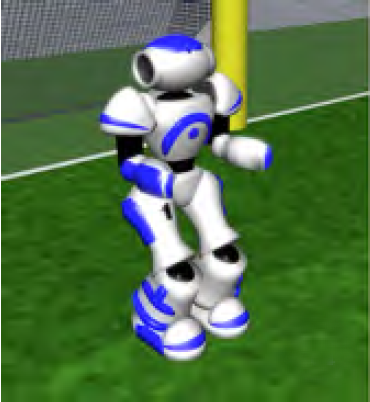
\includegraphics[width=0.15\textwidth]{images/initial_pose.png}}
    \caption{Initial pose.}
    \label{fig:initial_pose}
\end{figure}

The robot's objective is to run as fast as possible, in a straight line, and the reward is based on it's torso's x-coordinate difference
from the last step. The more the robot runs, the higher the reward.

The stopping behaviour was only trained after optimizing the running behaviour.
The robot is placed in the same initial pose as before, and runs for some time until the stopping behaviour is triggered.


\section{Methodology}\label{Methodology}

\section{Simulator and Agent}\label{Simulator and Agent}

\section{State and Action Space}\label{State and Action Space}

\section{Results and Discussion}\label{Results and Discussion}

\section{Conclusions and Future Work}\label{Conclusions and Future Work}

\section{Acknowledgments}\label{Acknowledgments}

\begin{thebibliography}{00}
    \bibitem{lau2020fc}Lau, N., Reis, L., Simoes, D., Abreu, M., Silva, T. \& Resende, F. FC Portugal 3D Simulation Team: Team Description Paper 2020.  (2023)
    \bibitem{10.1007/978-3-030-35699-6_1}Abreu, M., Reis, L. \& Lau, N. Learning to Run Faster in a Humanoid Robot Soccer Environment Through Reinforcement Learning. {\em RoboCup 2019: Robot World Cup XXIII}. pp. 3-15 (2019)
    \bibitem{naorobot} Nao the Humanoid and Programmable Robot, \href{www.aldebaran.com/en/nao}{www.aldebaran.com/en/nao}. Last accessed 24 Dec 2023
    \bibitem{robocup97} Noda, I., Suzuki, S. J., Matsubara, H., Asada, M., Kitano, H.: RoboCup-97: The first robot world cup soccer games and conferences. AI magazine 19(3), 49-49 (1998)
\end{thebibliography}

\end{document}
